\section{Pentago}
\label{Pentago}
Pentago is a two-player abstract strategy game invented by Tomas Flodén. The American Company MindtwisterUSA [1] has the rights of developing and commercializing the product in North America. %http://www.mindtwisterusa.com/product/classic-wood-pentago


\begin{wrapfigure}{r}{0.5\textwidth}
  \begin{center}
    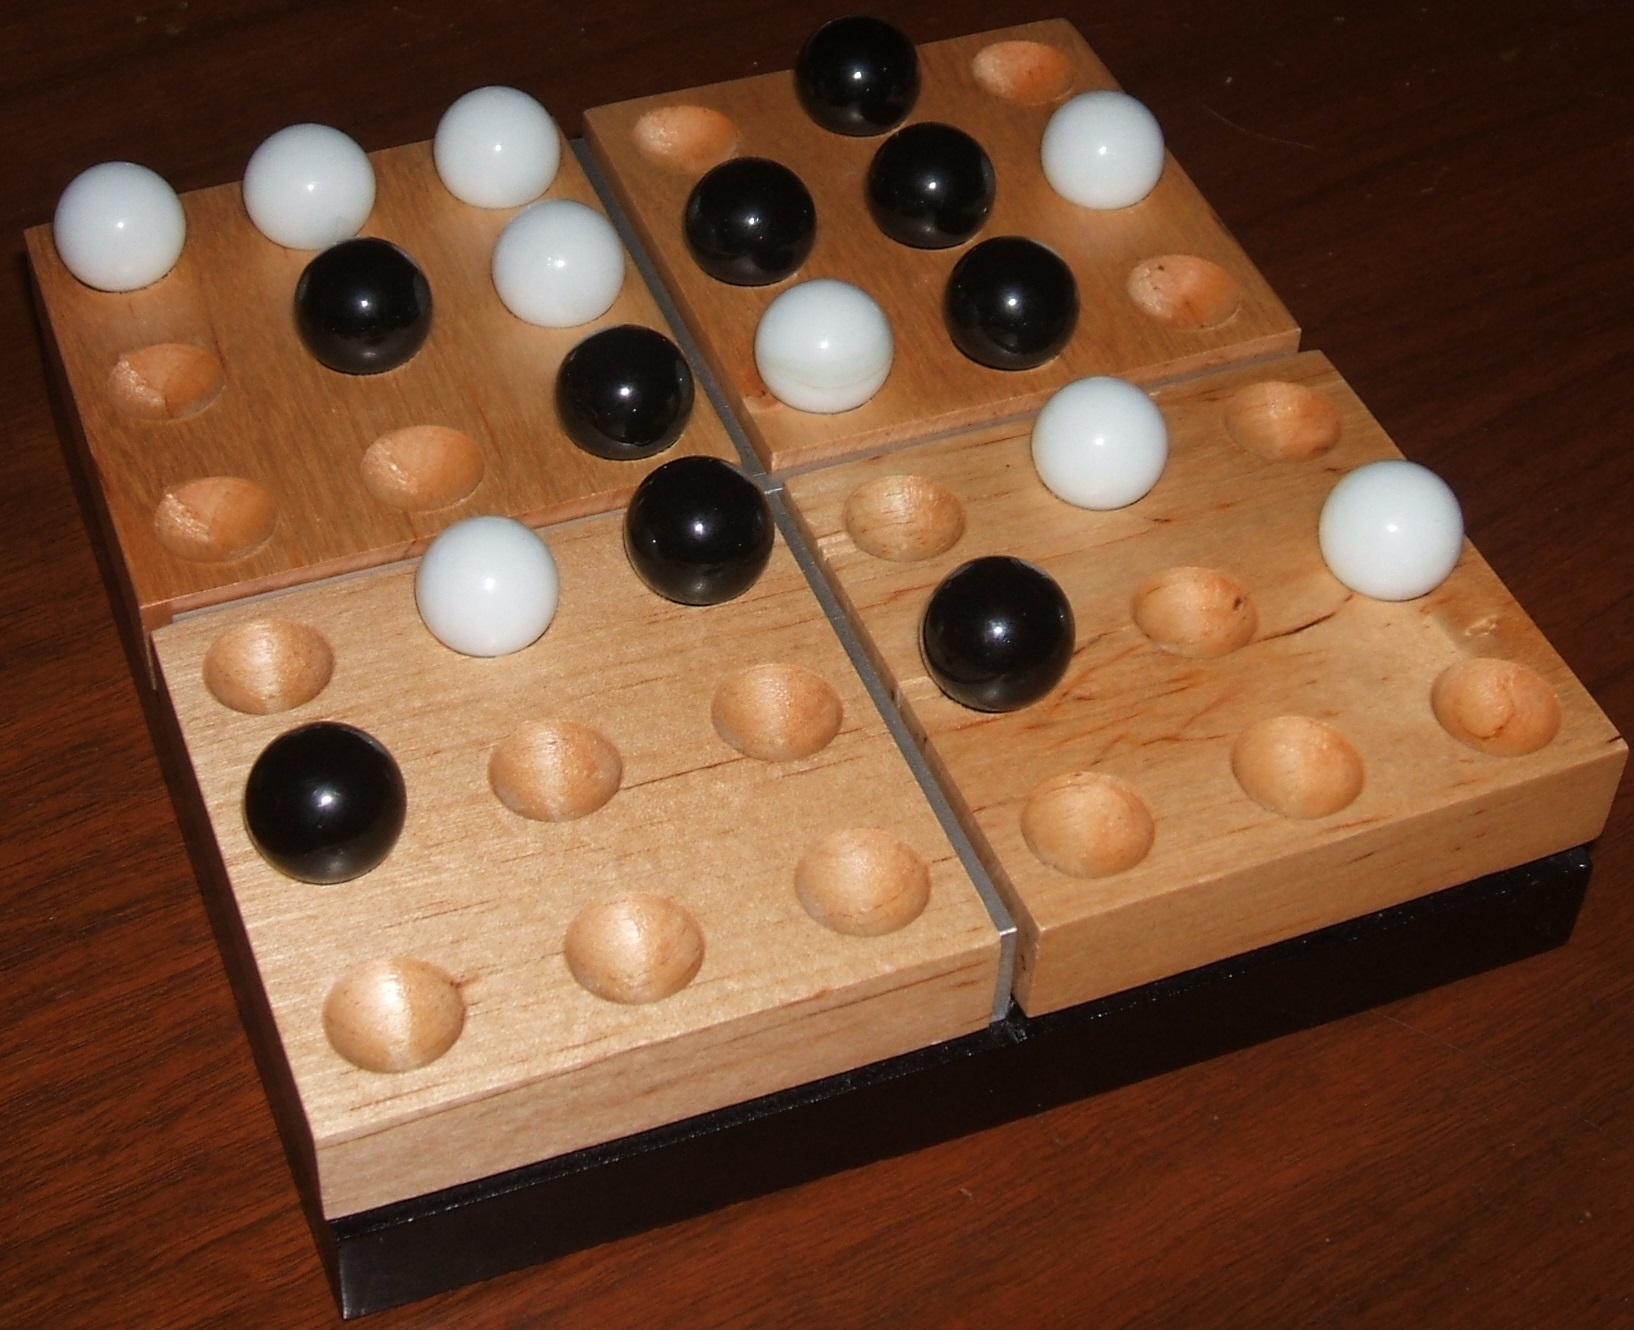
\includegraphics[width=0.48\textwidth]{Images/Pentago-Game-Winning-Position.jpg}
  \end{center}
  \caption{The pentago board}
  \label{fig:boardpic}
\end{wrapfigure}

The game is played on a 6×6 board divided into four 3×3 sub-boards (or quadrants). Taking turns, the two players place a marble of their color (either black or white) onto an unoccupied space on the board, and then rotate one of the sub-boards by 90 degrees either clockwise or anti-clockwise. This is optional in the beginning of the game, up until every sub-board no longer has rotational symmetry, at which point it becomes mandatory (this is because until then, a player could rotate an empty sub-board or one with just a marble in the middle, either of which has no real effect). A player wins by getting five of their marbles in a vertical, horizontal or diagonal row (either before or after the sub-board rotation in their move). If all 36 spaces on the board are occupied without a row of five being formed then the game is a draw. %add wikipedia reference
